\section{Evaluation} \label{sec:peregrine-eval}

\begin{table*}[t]
\small
\begin{center}
{
\begin{tabular}{cp{.78\textwidth}}
{\bf Program} & {\bf Race Description} \\
\hline

\apache & Reference count decrement and check against 0 are not atomic,
resulting in a program crash.\\

\pbzip & Variable \vv{fifo} is used by one thread after being freed by
another thread, resulting in a program crash.\\

\barnes & Variable \vv{tracktime} is read by one thread before assigned the
correct value by another thread.\\

\fft & \vv{initdonetime} and \vv{finishtime} are read by one thread before
assigned the correct values by another thread.\\

\lun & Variable \vv{rf} is read by one thread before assigned the correct
value by another thread. \\

\streamcluster & \parsec has a custom barrier implementation that
synchronizes using a shared integer flag \vv{is\_arrival\_phase}.
% One write to the flag is protected by mutex but one read from it is not.
\\

\racey & Numerous intentional races caused by multiple threads reading and
writing global arrays \vv{sig} and \v{m} without synchronization. \\

\end{tabular}}
\end{center}
\vspace{-.2in}
\caption{{\em Programs used for evaluating \peregrine's
    determinism}.} \label{table:races}
\vspace{-.1in}
\end{table*}


Our \peregrine implementation consists of 29,582 lines of C++ code, including
1,338 lines for the recorder; 2,277 lines for the replayer; and 25,967 lines
for the analyzer.  The analyzer further splits into 7,845 lines for
determinism-preserving slicing, 12,332 lines for schedule-guided
simplification, and 5,790 lines for our LLVM frontend to \vv{bddbddb}.

% TODO describe all programs
We evaluated our \peregrine implementation on a diverse set of \peregrinenprog programs,
including \apache, a popular web server; \pbzip, a parallel compression
utility; \aget, a parallel \vv{wget}-like utility; \pfscan, a parallel
\vv{grep}-like utility; parallel implementations of 13
computation-intensive algorithms, 10 in \splash and 3 in \parsec; and
\racey, a benchmark specifically designed to exercise deterministic
execution and replay systems~\cite{racy-stress}.  All \splash benchmarks
were included except one that we cannot compile, one that our current prototype
cannot handle due to an implementation bug, and one that does not run
correctly in 64-bit environment.  The chosen \parsec benchmarks
(\blackscholes, \swaptions and \streamcluster) include the ones that (1)
we can compile, (2) use threads, and (3) use no x86 inline assemblies.
These programs were widely used in previous studies (\eg,~\cite{lu:concurrency-bugs,syncfinder:osdi10,grace:oopsla09}).

Our evaluation machine was a 2.67 GHz dual-socket quad-core Intel Xeon
machine with 24 GB memory running Linux 2.6.35.  When evaluating \peregrine on
\apache and \aget, we ran the evaluated program on this machine and the
corresponding client or server on another to avoid contention
between the programs.  These machines were connected via 1Gbps LAN.  We
compiled all programs to machine code using \vv{llvm-gcc -O2} and the
LLVM compiler \vv{llc}.  We used eight worker threads for all
experiments.

Unless otherwise specified, we used the following workloads in our
experiments.  For \apache, we used \ab~\cite{apachebench} to repeatedly
download a 100~KB webpage. For \pbzip, we compressed a 10~MB randomly
generated text file.
For \aget, we downloaded a 77~MB file (\vv{Linux-3.0.1.tar.bz2}). 
For \pfscan, we scanned the keyword \vv{return} from 100 randomly chosen
files in GCC.  For \splash and \parsec programs, 
we ran workloads which typically completed in 1-100 ms.

In the remainder of this section, we focus on four questions:
\begin{enumerate}

\item[\S\ref{sec:peregrine-deterministic}:] Is \peregrine deterministic if there are
  data races?  Determinism is one of the strengths of \peregrine over the
  sync-schedule approach.

\item[\S\ref{sec:peregrine-efficient}:] Is \peregrine fast?  For typical multithreaded
  programs that have rare data races, \peregrine should be roughly as fast as
  the sync-schedule approach.  Efficiency is one of the strengths of \peregrine
  over the mem-schedule approach.

\item[\S\ref{sec:peregrine-stable}:] Is \peregrine stable? That is, can it frequently
  reuse schedules?  The higher the reuse
  rate, the more repeatable program behaviors become and the more \peregrine can
  amortize the cost of computing hybrid schedules.

\item[\S\ref{sec:peregrine-annotation}:] Can \peregrine significantly reduce manual
  annotation overhead?  Recall that our previous
  work~\cite{cui:tern:osdi10} required developers to manually annotate the
  input affecting schedules.

\end{enumerate}

\subsection{Determinism} \label{sec:peregrine-deterministic}



We evaluated \peregrine's determinism by checking whether \peregrine could
deterministically resolve races.  Table~\ref{table:races} lists the seven
racy programs used in this experiment.  We selected the first five because
they were frequently used in previous
studies~\cite{avio:asplos06,ctrigger:asplos09,lu:concurrency-bugs,pres:sosp09}
and we could reproduce their races on our evaluation machine.  We selected the
integer flag race in \parsec to test whether \peregrine can handle ad hoc
synchronization~\cite{syncfinder:osdi10}.  We selected \racey to stress
test \peregrine: each run of \racey may have thousands of races, and if any of
these races is resolved differently, \racey's final output changes
with high probability~\cite{racy-stress}.

\begin{table}[t]
\small
\centering
\begin{tabular}{ccc}
{\bf Program} & {\bf Races} & {\bf Order Constraints} \\
\hline
\apache  & 0 & 0 \\
\pbzip   & 4 & 3 \\
\barnes  & 5 & 1 \\
\fft     & 10 & 4 \\
\lun      & 10 & 7 \\
\streamcluster & 0 & 0 \\
\racey   & 167974 & 9963 \\
\end{tabular}
\caption{{\em Hybrid schedule statistics.} Column {\bf Races} shows the
  number of races detected according the corresponding
  sync-schedule, and Column {\bf Order Constraints} shows the number of execution
  order constraints \peregrine adds to the final hybrid schedule.  The latter
  can be smaller than the former because \peregrine prunes subsumed execution
  order constraints (\S\ref{sec:peregrine-schedule}).  \peregrine detected no races for
  \apache and \streamcluster because the corresponding sync-schedules are
  sufficient to resolve the races deterministically; it thus adds no order
  constraints for these programs.} \label{tab:peregrine-racy-edges}
\end{table}

For each program with races, we recorded an execution trace and computed a
hybrid schedule from the trace.  Table~\ref{tab:peregrine-racy-edges} shows for each
program (1) the number of dynamic races detected according to the
sync-schedule and (2) the number of execution order constraints in the
hybrid schedule.  The reduction from the former to the latter shows how
effectively \peregrine can prune redundant order constraints
(\S\ref{sec:peregrine-schedule}).  In particular, \peregrine prunes 94\% of the constraints
for \racey.  For \apache and
\streamcluster, their races are already resolved deterministically by
their sync-schedules, so \peregrine adds no execution order
constraints.

To verify that the hybrid schedules \peregrine computed are deterministic, we
first manually inspected the order constraints \peregrine added for each program
except \racey (because it has too many races for manual verification).  Our
inspection results show that these constraints are sufficient to resolve
the corresponding races.  We then re-ran each program including \racey 1000
times while enforcing the hybrid schedule and injecting delays; 
and verified that each run reused the schedule and computed equivalent results.
(We determined result equivalence by checking either the output or whether
the program crashed.)


\newcommand{\bad}{\ding{54}\xspace}
\newcommand{\good}{\ding{52}\xspace}

\begin{table}[t]
\small
\centering
\begin{tabular}{ccc}
\multirow{2}{*}{\bf Program} & \multicolumn{2}{c}{\bf Deterministic?} \\
& {\bf sync-schedule} & {\bf hybrid schedule} \\
\hline
\apache  & \good & \good \\
\pbzip   & \bad  & \good \\
\barnes  & \bad  & \good \\
\fft     & \bad  & \good \\
\lun      & \bad  & \good \\
\streamcluster  & \good  & \good \\
\racey   & \bad  & \good \\
\end{tabular}
\vspace{-.05in}
\caption{{\em Determinism of sync-schedules v.s. hybrid
    schedules.}} \label{tab:peregrine-determinism}
\vspace{-.1in}
\end{table}

We also compared the determinism of \peregrine to our previous work~\cite{cui:tern:osdi10} which
only enforces sync-schedules.  Specifically, we reran the seven programs with
races 50 times enforcing only the sync-schedules and injecting delays,
and checked whether the reuse runs computed equivalent
results as the recorded run.  As shown in Table~\ref{tab:peregrine-determinism},
sync-schedules are unsurprisingly deterministic for \apache and
\streamcluster, because no races are detected according to the
corresponding sync-schedules.  However, they are not
deterministic for the other five programs, illustrating
one advantage of \peregrine over the sync-schedule approach.

\subsection{Efficiency} \label{sec:peregrine-efficient}

% We show numbers from our previous work~\cite{cui:tern:osdi10} and
% CoreDet~\cite{coredet:asplos10} for reference.

\para{Replayer overhead.}  The most performance-critical component is the
replayer because it operates within a deployed program.
Figure~\ref{fig:peregrine-overhead} shows the execution times when reusing hybrid
schedules; these times are normalized to the nondeterministic
execution time.  (The next paragraph compares these times to those of
sync-schedules.)  For \apache, we show the throughput (TPUT) and response
time (RESP).  All numbers reported were averaged over 500 runs.  \peregrine
has relatively high overhead on \watern (22.6\%) and \cholesky (46.6\%)
because these programs do a large number of mutex operations within tight loops.
Still, this overhead is
% of \peregrine on these programs and workloads is below 46\%,
lower than the reported 1.2X-6X overhead of a mem-schedule DMT
system~\cite{coredet:asplos10}.  Moreover, \peregrine speeds up \barnes, \lun,
\radix, \waters, and \ocean (by up to 68.7\%) because it safely skips
synchronization and sleep operations (\S\ref{sec:peregrine-nowait}).  For the other
programs, \peregrine's overhead or speedup is within 15\%.  (Note that
increasing the page or file sizes of the workload
tends to reduce \peregrine's relative overhead
because the network and disk latencies dwarf \peregrine's.)

\begin{figure}[t]
\centering
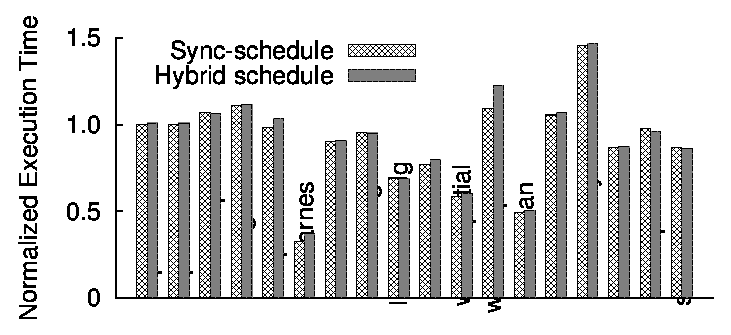
\includegraphics[width=0.9\columnwidth]{peregrine/figures/overhead.eps}
\vspace{-.3in}
\caption{{\em Normalized execution time when reusing sync-schedules
    v.s. hybrid schedules.}  A time value greater than 1
  indicates a slowdown compared to a nondeterministic execution without
  \peregrine.  We did not include \racey because it was not designed for
  performance benchmarking. } \label{fig:peregrine-overhead}
\end{figure}

For comparison, Figure~\ref{fig:peregrine-overhead} shows the normalized
execution time when enforcing just the sync-schedules.  This overhead is
comparable to our previous work~\cite{cui:tern:osdi10}.  For all
programs except \watern, the overhead of enforcing hybrid schedules is only slightly
larger (at most 5.4\%) than that of enforcing sync-schedules.
This slight increase comes from two sources: (1) \peregrine has to enforce
execution order constraints to resolve races deterministically for \pbzip,
 \barnes, \fft, and \lun; and (2) the instrumentation framework \peregrine uses
also incurs overhead (\S\ref{sec:peregrine-enforce-schedule}). 
The overhead for \watern increases by 13.4\% because it calls functions
more frequently than the other benchmarks, and our instrumentation framework
inserts code at each function entry and return
(\S\ref{sec:peregrine-enforce-schedule}).


\begin{figure}[b!]
\centering
\includegraphics[width=\columnwidth]{peregrine/figures/opt.eps}
\vspace{-.3in}
\caption{{\em Speedup of optimization techniques.} Note that Y axis is
  broken.} \label{fig:peregrine-opt}
\end{figure}

Figure~\ref{fig:peregrine-opt} shows the speedup of flag relay
(\S\ref{sec:peregrine-enforce-schedule}) and skipping blocking operations
(\S\ref{sec:peregrine-nowait}).  Besides \watern and \cholesky, a
second group of programs, including \barnes, \lun, \radix, \waters, and
\ocean, also perform many synchronization operations, so flag relay speeds up
both groups of programs significantly.  Moreover, among the
synchronization operations done by the second group of programs, many are
\vv{pthread\_barrier\_wait()} operations, so \peregrine further speeds up these
programs by skipping these wait operations.



\begin{table}[!ht]
\scriptsize
\centering
\begin{tabular}{crrrrrrr}
{\bf Program} &{\bf Trace}&{\bf Det} & {\bf Sli}  & {\bf Sim} & {\bf Sym} \\
\hline                                                                   
\apache       & 449       & 0.4      & 885.32     & n/a       & 5.8       \\
\pbzip        & 2,227     & 0.1      & 587.9      & 317.8     & 19.7      \\
\aget         & 233       & 0.4      & 78.8       & 60.1      & 13.2      \\
\pfscan       & 46,602    & 1.1      & 1,601.4    & 2,047.9   & 1,136.6   \\
\barnes       & 324       & 0.2      & 300.5      & 481.5     & 56.9      \\
\fft          & 39        & 0.0      & 2.1        & 3,661.7   & 0.4       \\
\luc          & 44,799    & 19.9     & 1,271.5    & 124.9     & 1,126.7   \\
\lun          & 41,302    & 21.2     & 1,999.8    & 14,243.8  & 1,201.0   \\
\radix        & 3,110     & 1.5      & 46.2       & 96.4      & 182.9     \\
\waters       & 7,508     & 1.0      & 1,407.0    & 9,628.1   & 120.6     \\
\watern       & 12,381    & 1.7      & 962.3      & 1,841.4   & 215.7     \\
\ocean        & 55,247    & 26.4     & 2,259.3    & 5,902.8   & 2,062.1   \\
\fmm          & 13,772    & 8.3      & 260.5      & 1,107.5   & 151.3     \\
\cholesky     & 47,200    & 28.8     & 3,102.9    & 6,350.1   & 685.5     \\
\blackscholes & 62,024    & 16.5     & 539.9      & 542.9     & 3,284.8   \\
\swaptions    & 1,366     & 0.0      & 23.2       & 87.3      & 1.2       \\
\streamcluster& 259       & 0.1      & 1.4        & 1.9       & 4.9       \\ 
\end{tabular}
\caption{{\em Analysis time.} {\bf Trace} shows the number of thousand
  LLVM instructions in the execution trace of the evaluated programs,
  the main factor affecting the execution time of \peregrine's various analysis
  techniques, including race detection ({\bf Det}), slicing ({\bf Sli}),
  simplification and alias analysis ({\bf Sim}), and symbolic execution
  ({\bf Sym}).  The execution time is measured in seconds.  The \apache
  trace is collected from one window of eight requests.  \apache uses
  thread pooling which our simplification technique currently does not
  handle well (\S\ref{sec:peregrine-window}); nonetheless, slicing without simplification
  works reasonably well for \apache already
  (\S\ref{sec:peregrine-stable}).} \label{tab:peregrine-analysis-overhead}
\end{table}


\para{Analyzer and recorder overhead.}  Table~\ref{tab:peregrine-analysis-overhead}
shows the execution time of \peregrine's various program analyses.  The
execution time largely depends on the size of the execution trace.  All
analyses typically finish within a few hours.  For \pbzip and \fft, we
used small workloads (compressing 1~KB file and transforming a 256X256
matrix) to reduce analysis time and to illustrate that the schedules
learned from small workloads can be efficiently reused on large workloads.
The simplification and alias analysis time of \fft is large compared to its
slicing time because it performs many multiplications on array indexes,
slowing down our range analysis.  Although \lun and \luc implement the
same scientific algorithm, their data access patterns are very different
(\S\ref{sec:peregrine-stable}), causing \peregrine to spend more time analyzing \lun than \luc.

\begin{figure}[b!]
\centering
\includegraphics[width=.7\columnwidth]{peregrine/figures/new-recorder.eps}
\vspace{-.25in}
\caption{{\em Overhead of recording \vv{load} and \v{store} instructions.}} \label{fig:peregrine-new-recorder-overhead}
\end{figure}

As discussed in \S\ref{sec:peregrine-record}, \peregrine currently runs \klee to record
executions.  Column Sym is also the overhead of \peregrine's recorder.  This
crude, unoptimized recorder can incur large slowdown compared to
the normal execution of a program.  However, this slowdown can be reduced
to around 10X using existing record-replay
techniques~\cite{idna:vee06,scribe:sigmetrics10}.  Indeed, we have
experimented with a preliminary version of a new recorder that records an
execution by instrumenting \vv{load} and \v{store} instructions and saving
them into per-thread logs~\cite{idna:vee06}.  Figure~\ref{fig:peregrine-new-recorder-overhead} shows that
this new recorder incurs roughly 2-35X slowdown on eight programs,
comparable to existing record-replay systems.  Due to time
constraints, we have not integrated this new recorder with \peregrine.



\subsection{Stability} \label{sec:peregrine-stable}

Stability measures how frequently \peregrine can reuse schedules.  The more
frequently \peregrine reuses schedules, the more efficient it is, and the
more repeatable a program running on top of \peregrine becomes.  While \peregrine
achieves determinism and efficiency through hybrid schedules, it may have
to pay the cost of slightly reduced reuse rates compared to a
manual approach~\cite{cui:tern:osdi10}.




\begin{figure}[t]
\centering
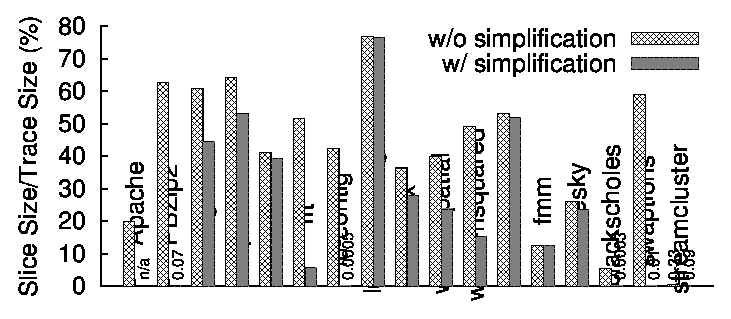
\includegraphics[width=\columnwidth]{peregrine/figures/slicing.eps}
\vspace{-.3in}
\caption{{\em Slicing ratio after applying determinism-preserving slicing alone 
    (\S\ref{sec:peregrine-slice}) and after further applying schedule-guided
    simplification (\S\ref{sec:peregrine-guide}).}} \label{fig:peregrine-slice-ratio}
\vspace{-.05in}
\end{figure}

A key factor determining \peregrine's schedule-reuse rates is how effectively it
can slice out irrelevant instructions from the execution traces.
Figure~\ref{fig:peregrine-slice-ratio} shows the ratio of the slice size over the trace size for
\peregrine's determinism-preserving slicing technique, with and without
schedule-guided simplification.  The slicing technique alone reduces the
trace size by over 50\% for all programs except \pbzip, \aget, \pfscan,
\fft, \lun, \ocean, and \swaptions.  The slicing technique combined with
scheduled-guide simplification vastly reduces the trace size for \pbzip,
\aget, \fft, \luc, and \swaptions.

Recall that \peregrine computes the preconditions of a schedule from
the input-dependent branches in a trace slice.  The
fewer branches included in the slice, the more general the preconditions
\peregrine computes tend to be.  We further measured the number of such
branches in the trace slices.  Table~\ref{tab:peregrine-slice-ratio} shows the
results, together with a upper bound determined by the total number of
input-dependent branches in the execution trace, and a lower bound
determined by only including branches required to reach the recorded
synchronization operations.  This lower bound may not be tight as we ignored data
dependency.  For \barnes, \fft, \blackscholes, \swaptions, and
\streamcluster, slicing with simplification (Column ``Slicing+Sim'')
achieves the best possible reduction.  For \pbzip, \aget, \pfscan, and \luc, the
number of input-dependent branches in the trace slice is close to the
lower bound.  In the remaining programs, \apache, \fmm, and \cholesky
also enjoy large reduction, while the other five programs do not.  This table
also shows that schedule-guided simplification is key to reduce the
number of input-dependent branches for \pbzip, \fft, \luc, \blackscholes, 
and \swaptions,
and to reach the lower bound for \blackscholes, \swaptions, and \streamcluster.


We manually examined the preconditions \peregrine computed from the
input-dependent branches for these programs.  We category these programs
below.

\para{Best case}: \pbzip, \fft, \luc, \blackscholes, \swaptions,
  and \streamcluster. For these programs, \peregrine computes the weakest
  (\ie, most relaxed) preconditions. The preconditions often allow \peregrine
  to reuse one or two schedules for each number of threads, putting no
   or few constraints on the data processed.
  Schedule-guided simplification is crucial for
  these programs; without simplification, the preconditions
  would fix the data size and contents.

\para{Slicing limitation}: \apache and \aget. The
  preconditions \peregrine computes for \apache fix the URL length; they also
  constrain the page size to be within an 8~KB-aligned range if
    the page is not cached.  The preconditions \peregrine computes for \aget fix
    the positions of ``\vv{/}'' in the URL and narrow down the file size
    to be within an 8~KB-aligned range.  These preconditions thus
      unnecessarily reduce the schedule-reuse rates.  Nonetheless, they
      can still match many different inputs, because they do not constrain
      the page or file contents.

\para{Symbolic execution limitation}: \barnes.  \barnes
  reads in two floating point numbers from a file, and their values affect
  schedules.  Since \peregrine cannot symbolically execute floating point
  instructions, it currently does not collect preconditions from them.

\para{Alias limitation}: \lun, \radix, \waters, \watern, \ocean,
  and \cholesky.  Even with simplification, \peregrine's alias analysis
  sometimes reports may-alias for pointers accessed in different threads,
  causing \peregrine to include more instructions than necessary in the
  slices and compute preconditions that fix the input data.  For
  instance, each thread in \lun accesses disjoint regions in a global
  array, but the accesses from one thread are \emph{not} continuous,
  confusing \peregrine's alias analysis.  (In contrast, each thread in \luc accesses
  a contiguous array partition.)

\para{Programs that rarely reuse schedules}: \pfscan and
  \fmm.  For instance, \pfscan searches a keyword in a set of files using
  multiple threads, and for each match, it grabs a lock to increment a
  counter.  A schedule computed on one set of files is unlikely to suit
  another.

\begin{table}[!ht]
\small
\centering
\begin{tabular}{crrrr}
\multirow{2}{*}{\bf Program} & \multirow{2}{*}{\bf UB} 
& \multicolumn{2}{c}{\bf \peregrine} 
& \multirow{2}{*}{\bf LB} \\
& & {\bf Slicing} & {\bf Slicing+Sim} & \\
\hline
\apache       &  4,522   &  624    & n/a      & 56     \\
\pbzip        &  913     &  865    & 101      & 94     \\
\aget         & 20,826   & 18,859  & 9,514    & 9,491  \\
\pfscan       & 1,062,047& 992,524 & 992,520  & 992,501\\
\barnes       &  92      & 52      & 52       & 52     \\
% This is fft -p8 -m6 slicing results, not m16. Range analysis currently can not run m16.
\fft          &  2,266   & 1,568   & 17       & 17     \\
\luc          &2,823,379 &2,337,431& 131      & 128    \\
\lun          &2,962,621 &2,877,877& 2,876,364& 128    \\
\radix        &  175,679 & 98,750  & 89,732   & 75     \\
\waters       &  98,054  & 77,567  & 76,763   & 233    \\
\watern       &  89,348  & 76,786  & 76,242   & 1,843  \\
\ocean        &2,605,185 &2,364,538&2,361,256 & 400    \\
\fmm          &  299,816 & 57,670  & 56,532   & 1,642  \\
\cholesky     &  7,459   & 1,627   & 1,627    & 1,233   \\
\blackscholes & 421,909  & 409,618 & 10       & 10 \\
\swaptions    & 35,584   & 35,005  & 21       & 21 \\
\streamcluster& 20,851   & 75      & 42       & 42 \\
\end{tabular}
\vspace{-.1in}
\caption{{\em Effectiveness of program analysis techniques.}  {\bf UB}
  shows the total number of input-dependent branches in the
  corresponding execution trace, an upper bound on the number included in 
  the trace slice.  {\bf Slicing} and {\bf Slicing+Sim} show the
  number of input-dependent branches in the slice after applying
  determinism-preserving slicing alone (\S\ref{sec:peregrine-slice}) and after
  further applying schedule-guided simplification
  (\S\ref{sec:peregrine-guide}). {\bf LB} shows a lower bound on the number of
  input-dependent branches, determined by only including branches
  required to reach the recorded synchronization operations.
  This lower bound may not be tight as we ignored data
  dependency when computing it.} \label{tab:peregrine-slice-ratio}
\vspace{-.05in}
\end{table}




\subsection{Ease of Use} \label{sec:peregrine-annotation}

\begin{table}[!ht]
\centering
\small
\begin{tabular}{crcc}
{\bf Program} & {\bf LOC} & {\bf \peregrine} & {\bf \tern} \\
\hline
% -6.0 
\apache       & 464~K   & 24  & 6  \\
\pbzip        & 7,371  & 1   & 3  \\
\aget         &   834  & 0   & n/a\\
\pfscan       &   776  & 0   & n/a\\
\barnes       & 1,954  & 0   & 9  \\
\fft          & 1,403  & 1   & 4  \\   
\luc          & 991    & 0   & n/a  \\ 
\lun          & 1,265  & 0   & 3  \\   
\radix        & 661    & 0   & 4  \\   
\waters       & 1,573  & 0   & 9  \\
\watern       & 1,188  & 0   & 10 \\
\ocean        & 6,494  & 0   & 5  \\
\fmm          & 3,208  & 0   & 9  \\
\cholesky     & 3,683  & 0   & 4  \\
\blackscholes & 1,275  & 0   & n/a\\
\swaptions    & 1,110  & 0   & n/a\\
\streamcluster& 1,963  & 0   & n/a\\
\racey        & 124    & 0   & n/a\\
\end{tabular}
\vspace{-.05in}
\caption{{\em Source annotation requirements of \peregrine v.s. \tern.}  {\bf
    \peregrine} represents the number of annotations added for \peregrine, and {\bf
    \tern} counts annotations added for \tern.  Programs not included in
  the \tern evaluation are labeled n/a. LOC of \pbzip also includes the
  lines of code of the compression library \vv{libbz2}.} \label{table:peregrine-apps}
\vspace{-.05in}
\end{table}

Table~\ref{table:peregrine-apps} shows the annotations (\S\ref{sec:peregrine-func-summary}) we
added to make the evaluated programs work with \peregrine.  For most programs,
\peregrine works out of the box.  \apache uses its own library functions for
common tasks such as memory allocation, so we annotated 21 such
functions.  We added two annotations to mark the boundaries of client
request processing and one to expose the hidden state
in \apache (\S\ref{sec:peregrine-window}).  \pbzip decompression
uses a custom search function (\vv{memstr}) to scan through the input file
for block boundaries.  We added one annotation for this function to relax
the preconditions \peregrine computes.  (\peregrine works automatically with \pbzip
compression.)  We added one assertion to annotate the range of a variable
in \fft (\S\ref{sec:peregrine-func-summary}).

For comparison, Table~\ref{table:peregrine-apps} also shows the annotation overhead of our previous DMT system \tern~\cite{cui:tern:osdi10}.  For all programs except \apache, \peregrine
has fewer number of annotations than \tern.  Although the number
of annotations that \tern has is also small, adding these annotations may
require developers to manually reconstruct the control- and
data-dependencies between instructions.


% emphasize interesting side effects
In order to make the evaluated programs work with \peregrine, we had to fix several bugs
in them.  For \aget, we fixed an off-by-one write in \vv{revstr()} which
prevented us from tracking constraints for the problematic write, and a
missing check on the return value of \vv{pwrite()} which prevented us from
computing precise ranges.  We fixed similar missing checks in \swaptions,
\streamcluster, and \radix.  We did not count these modifications in
Table~\ref{table:peregrine-apps} because they are real bug fixes.  (This interesting
side-effect illustrates the potential of \peregrine as an error detection tool:
the precision gained from simplification enables \peregrine to detect real races
in well-studied programs.)


